\documentclass{article}
\usepackage{graphicx}
\usepackage{amsmath}
\graphicspath{{images/}}



\begin{document}

\begin{flushright}
        {\scriptsize \textbf{Facultad de Matemática y Computación}}
        
\includegraphics[width=4cm, height=4cm]{matcom.jpg}\\
    \end{flushright}
    
    \
    
    \
    
    \begin{center}
        \textbf{{\Huge PROYECTO DE }}
        
        \
    
        \textbf{{\Huge PROGRAMACIÓN I}}
        \
    
        \
         
        \
        
        \
        
\includegraphics[width = 10 cm ,height= 5 cm]{Screenshot 2023-07-17 at 15-44-54 The Logo Maker Built for 1000 Industries and 20M Users.png}\\
        \
    
        \
    
        \
    
        \textbf{{\Huge Moogle!}}
    \end{center}
    \begin{figure}[b]
        \begin{flushleft}
          \textit{\large Juan Miguel Maestre Rodriguez }
    
            \
        
            \textit{\large C-121}
        \end{flushleft}
    \end{figure}
    
\newpage
{\small
\textbf{\large Clase Normalize }
\\
Para normalizar los texto del proyecto se crea la clase Normalize en la cual se implementa el
método llamado Normalizing, a este se le pasara un valor de tipo “string” llamado “text”. Dentro
del método en la linea 9 a la variable “text” se le aplica el método ToLower el cual se le asigna a la
misma variable(Esto es porque el lenguaje CSharp es sensible a mayúsculas y minúsculas “Case
Sensitive” .Osea este lenguaje no interpreta de la misma forma “Perro” y “perro”).
\\

\centering
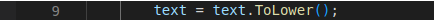
\includegraphics[height = 0.5 cm ]{Captura desde 2023-07-17 22-27-30.png}

\

Análogamente se utiliza la función $<$name$>$.Replace, en este caso text.Replace\\(“ á”, “ é ”, “ í ”, “ó” “ ú ” ) por las mismas pero sin tilde por la misma razón anterior (Case Sensitive) .

\ 

\centering
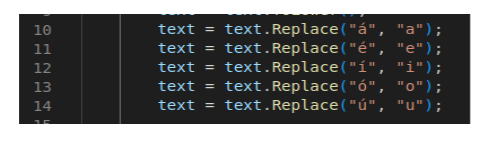
\includegraphics[height = 3 cm ]{Captura desde 2023-07-17 22-42-56.png}

\

Por ultimo se utiliza :

\

\centering
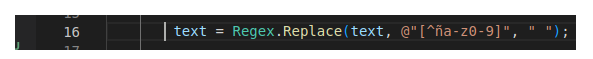
\includegraphics[height = 1.2 cm ]{Captura desde 2023-07-17 22-46-16.png}

\

Esta linea es para que todo lo que sea los caracteres que no están incluidos en ña-z0-9 sean
sustituidos por un espacio en blanco. Para esta función primero tenemos que importar la librería
System.Text.RegularExpressions;

\

\centering
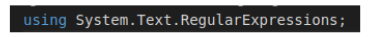
\includegraphics[height = 0.8 cm ]{Captura desde 2023-07-19 13-00-55.png}
\newpage
\textbf{\large CLase TF-IDF }

\

Para calcular el \textbf{TF-IDF} del proyecto se utiliza esta clase, pero primero que todo se tiene que saber que es TF-IDF(Term Frequency-Inverse Document Frecuency) frecuencia de término – frecuencia inversa de documento, 
es una medida numérica que expresa cuán relevante es una palabra para un documento en una colección.
Esta medida se utiliza a menudo como un factor de ponderación en la recuperación de información y la minería de texto

\

\begin{itemize}
\item\textbf{TF}: Cantidad de veces que se repite una palabra en el documento, entre la cantidad de palabras que contiene el documento. \\
\
\item\textbf{IDF}: Cantidad de documentos y Cantidad de documentos en los que aparece  una palabra.\\
\end{itemize}

\

El primero (\textbf{TF}) se calcula como  la cantidad de veces que se repite una palabra en el documento, entre la cantidad de palabras que contiene el documento.

\begin{equation*}
    TF = np / nd .
\end{equation*}

\

Donde :
\
\begin{itemize}
    \item\textbf{np} es la cantidad de veces que se repite una palabra en un documento\\
    \item\textbf{nd} es la cantidad de palabras que contiene el documento 
\\
\end{itemize}

\

La Frecuencia Inversa de Documento(\textbf{IDF}) se calcula como  Logaritmo en cuya base tiene la cantidad de documentos en los que aparece una palabra en específico y en su argumento la cantidad total  de documentos. 

\begin{equation*}
    IDF = \log{t/n}
\end{equation*}

\

Donde:
\\
\begin{itemize}
    \item\textbf{n} es la cantidad de documentos en los que aparece la palabra.
    \item\textbf{t} es la cantidad total de documentos  
\end{itemize}
\pagebreak
\textbf{\large DataBase }

\

En esta clase se forma la base de daos de Moogle Project.
Esta clase contiene el método llamado “Loading” al cual se le pasa una variable llamada “path” que es
de tipo “string” a la cual se le asigna el texto “Content” 

\

\centering

\includegraphics[height = 0.8 cm ]{Captura desde 2023-07-18 11-16-29.png}

\

En la línea 19 al array “directions” se le asigna el directorio de cada documento con la función 
Directory.GetFiles(Path.Join(“..” $<$variable$>$),””,SearchOption.AllDirectories);. 
A esta función se le pasó la variable path que tiene asignada la cadena de caracteres “Content”. 
Entonces esta encuentra la carpeta “Content” y después le asigna a cada posición del array la dirección de cada documento.

\

\centering

\includegraphics[height = 0.7 cm ]{Captura desde 2023-07-18 21-14-03.png}

\

En las líneas 20, 21, 22  a los arrays declarados anteriormente “nameDocuments” , “text” , “allwords”  
se le asigna la misma longitud de “directions” con la funcionalidad  $<$en este caso directions$>$.Lenght

\

\centering
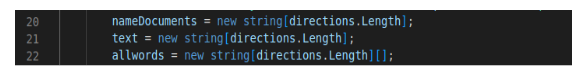
\includegraphics[height = 1.6 cm ]{Captura desde 2023-07-18 21-21-46.png}

\

En la línea 23 al array de diccionario que se había creado en con anterioridad le asignamos la misma longitud de “directions” respectivamente .

\

\centering
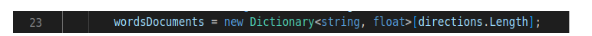
\includegraphics[height = 0.7 cm ]{Captura desde 2023-07-18 21-25-05.png}

\

En la línea 25 se creó un for en el cual se va iterando desde la primera posición del array “directions” por toda su longitud

\

\centering
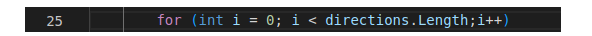
\includegraphics[height = 0.7 cm ]{Captura desde 2023-07-18 21-27-04.png}

\

En la linea 27 en cada iteración del for se le asigna al array nameDocuments en cada posición los nombres de cada documento guardado
en cada posición del array “directions”. Esto es gracias a la función  Path.GetFileNameWithoutExtension($<$en este caso directions[i]) 

\

\centering
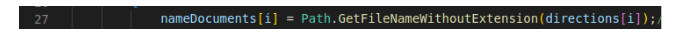
\includegraphics[height = 0.6 cm ]{Captura desde 2023-07-18 21-31-27.png}

\

En la linea 28 se aplica la función File.ReadAllText($<$en este caso directions[i]$>$). Este método abre los archivos correspondientes a 
los directorios guardados en cada posición del array “directions”, lee todo el texto de cada archivo y lo devuelve como una cadena. 
Después se le aplica el método “Normalizing” que está en la clase “Normalize” esto para normalizar el texto(En el sección de la clase 
Normalize se explica detalladamente cual es el objetivo de la misma) y después esto se guarda en cada posición del array text declarado
al principio de la clase. 

\

\centering
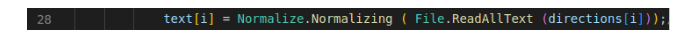
\includegraphics[height = 0.6 cm ]{Captura desde 2023-07-18 21-42-49.png}\\

\

En la línea 29 a cada posición del array “text” que contiene los textos de los documentos se normalizan: Primero con la función 
StringSplitOptions.RemoveEmptyEntries se eliminan los espacios en los textos y después con el método .Split se separa cada palabra 
por espacios en blanco y esto se le asigna al array allwords declarado en el principio. 

\

\centering
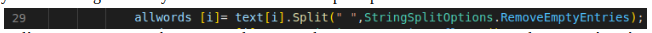
\includegraphics[height = 0.6 cm ]{Captura desde 2023-07-18 22-08-59.png}

\

La línea 30 tiene como objetivo que al ejecutar el programa no presente errores y diga qu está vacío.

\

\centering
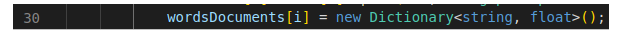
\includegraphics[height = 0.6 cm ]{Captura desde 2023-07-18 22-11-17.png}

\

De la línea 32 hasta la 39 se crea un foreach donde se va iterando por cada palabra de cada documento contenida en cada posición  del array allwords.
En la línea 34 se crea una condición donde si la palabra que está en los diccionarios de cada posición del array wordsDocuments está repetida entonces 
se suma 1 a un contador. Por cada repetición  Esto se hace con el objetivo de saber cuantas veces se repite cada palabra en un documento. En caso  
que la palabra se encuentre solo una vez en el documento se le asigna 1 . 

\

\centering
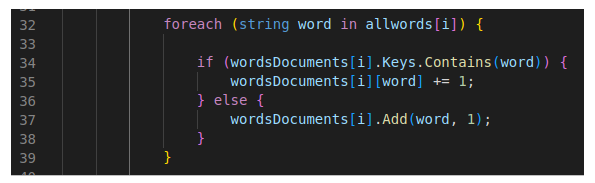
\includegraphics[height = 3.7 cm ]{Captura desde 2023-07-18 22-18-36.png}

\

De la línea 41 hasta la 44 se crea otro foreach donde se va iterando por cada posición del array allwords y entonces vamos a llamar  al método “TF” 
contenido en la clase TF-IDF y le vamos a pasar cada diccionario de cada posición del array “allwords” que contiene cada palabra del documento con 
la cantidad de veces que se repite en el mismo y también le vamos a pasar el valor de la cantidad de palabras que contiene el diccionario(Sé conoce 
que es un poco complejo de entender pero básicamente esto lo que hace es substituir el valor de repetición que contenía cada palabra del diccionario 
por su TF(En la clase se TF-IDF se explica qué es esto) ).

\

\centering
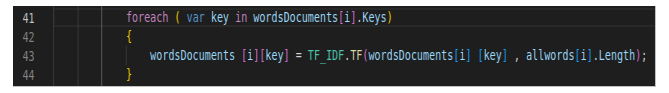
\includegraphics[height = 1.6 cm ]{Captura desde 2023-07-18 22-28-47.png}

\

\textbf{\large Clase Snippet }

\

Para introducir el Snippet en el proyecto se crea la clase publica Snippeten la cual se implementa el método llamado ShowWords a este se le pasará
un valor de tipo “string” llamado “text”. Dentro del método se crea una variable llamada “result” donde: Si la longitud del texto tiene mas de 
100 caracteres entonces en la variable se guardara un fragmento de hasta 100 caracteres, si no tiene una cantidad de caracteres superior a lo indicado 
anteriormente entonces se guardara el texto en su totalidad. Para poder guardar el fragmento de texto se utiliza el método [$<$palabra$>$.Substring($<$inicio$>$ , $<$final$>$)] .

\

\centering
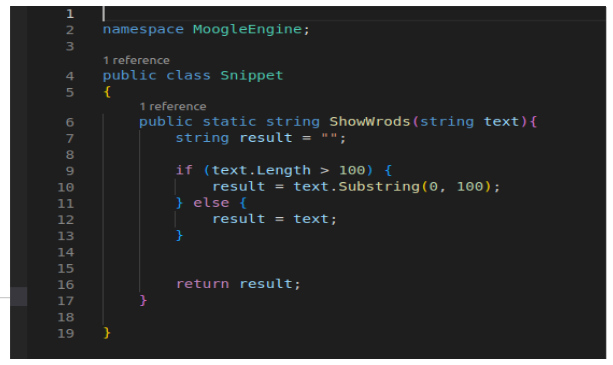
\includegraphics[height = 7.2 cm ]{Captura desde 2023-07-18 22-37-53.png}

\

\textbf{\large Clase Score }\\
Esta clase tiene como objetivo evaluar el nivel de importancia que tiene un documento según la búsqueda realizada. Para ello se crea un método público llamado “Ranking” 
se le pasará dos arrays uno de tipo string  “modify” y otro de tipo float  “IDF”.

\

\centering
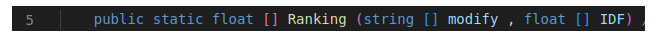
\includegraphics[height = 0.6 cm ]{Captura desde 2023-07-18 22-44-15.png}

\

En la línea 7 se crea un array de tipo float “ranking” al cual se le asigna el mismo tamaño del array “directions” creado en la clase DataBase. Para ello se utiliza 
(DataBase.directions.Lenght).

\

\centering
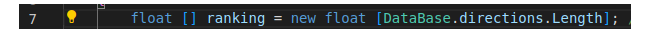
\includegraphics[height = 0.6 cm ]{Captura desde 2023-07-18 22-49-05.png}

\

En la línea 8 se crea una variable de tipo float llamada “tfxidf” a la que se le asigna temporalmente valor 0. 

\

\centering
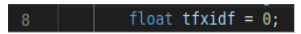
\includegraphics[height = 0.6 cm ]{Captura desde 2023-07-18 22-52-16.png}

\

En la línea 9 se crea un for en el que se se va iterando desde la posición 0 hasta el final del array de diccionarios  “wordsDocuments” . 

\

\centering
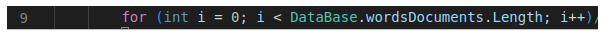
\includegraphics[height = 0.6 cm ]{Captura desde 2023-07-18 22-58-20.png}

\

En la línea 11 se crea una variable entera “j” y se le asigna valor 0.

\

\centering
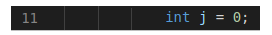
\includegraphics[height = 0.8 cm ]{Captura desde 2023-07-18 23-01-19.png}

\

De la línea 12 a la 24 se crea un foreach en el que vamos a iterar por cada “word” que contiene el array “modify” anteriormente declarado. Después se crea una condición
donde cada diccionario del array  de diccionarios “wordsDocuments” creado en la clase DataBase,si contiene la “word” de “modify” entonces se le agrega su nivel de 
importancia y coincidencia con “modify”(Esto es lo que se llama TF- IDF), ese valor se le asigna a la variable “tfxidf”. En caso de que no que no contenga la(s) palabra(s) 
se le resta valor. En la linea 27 se le asigna a cada posición de ranking el valor de “tfxidf” del documento en la posición que le corresponde. Y por ultimo en la línea 28
se vuelve a igualar a 0 la variable “tfxidf” para que su valor vuelva a reiniciarse y no hayan errores. 

\

\centering
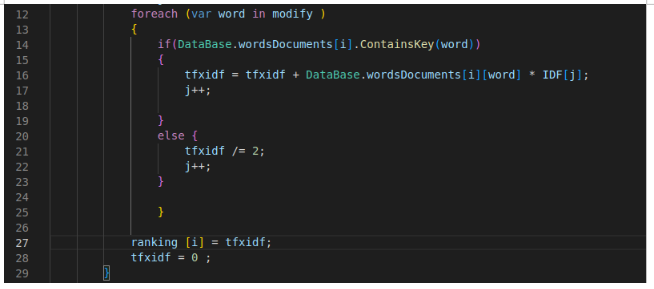
\includegraphics[height = 5.3 cm ]{Captura desde 2023-07-18 23-04-55.png}

\

\textbf{\large Clase Moogle }\\
Esta es la clase principal de Moogle Project  la cual se encarga de correr el programa. En las líneas 6 y 7 se crean dos diccionarios con los cuales se trabajará a continuación:

\

Posteriormente se crea el método ¨Query” el cual mostrará los resultados de los ingresado por el usuario en el Programa, a este se le pasa una variable de tipo string¨llamada “query¨ .

\

\centering
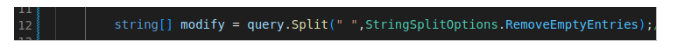
\includegraphics[height = 0.8 cm ]{Captura desde 2023-07-19 10-44-07.png}

\

En la línea 14 y 15 creamos dos arrays del mismo tamaño que ¨modify¨, el primero “count” va a ser un contador donde vamos a guardar la cantidad de documentos en los que aparece 
cada palabra de la query (Ej: Harry Potter… En la cantidad de documentos que se encuentra “Harry”, ese valor se guardará en la posición (0) de “count”). En el segundo “IDF” se 
almacenará los IDF de cada palabra de la query en su posición correspondiente 

\

\centering
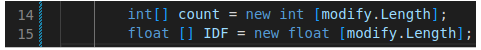
\includegraphics[height = 1 cm ]{Captura desde 2023-07-19 10-48-43.png}

\

De la línea 17 a la 25 se crean dos for, el primero itera desde la primera hasta la última posición de “modify” y el segundo igualmente pero de “text” contenido en la clase DataBase. 
Este  bloque de código tiene como objetivo que : si la palabra de la “query” está contenida en un documento se le suma 1 al contador(“count” array que se había declarado anteriormente, 
importante recordar que este  tiene el mismo tamaño  que “modify” por lo tanto almacenará la cantidad de repeticiones en la misma posición respectivamente ) .

\

\centering
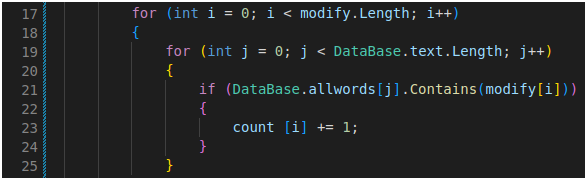
\includegraphics[height = 3.7 cm ]{Captura desde 2023-07-19 11-34-05.png}

\

De la línea 28 a la 31 se crea otro for el cual va a iterar desde la primera hasta la última posición de “modify”. Este bloque de código tiene como objetivo calcular los IDF de la “query”.
Para ello se llama al método “IDF” de la clase “TF-IDF” donde la cantidad de documentos será directions. Lenght y la cantidad en los cuales aparece la palabra es el contador(count). 

\

\centering
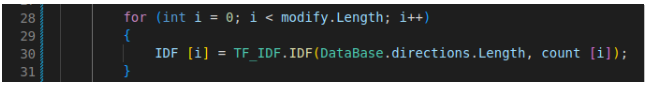
\includegraphics[height = 1.6 cm ]{Captura desde 2023-07-19 11-37-30.png}

\

En la línea 33 se crea un array de tipo tipo float llamado ranking, esta linea tiene como objetivo guardar “Score”(el nivel de concordancia de un documento con la query ) de cada documento.
Para ello se llama al método “Ranking” de la clase “Score” y se le pasan los arrays “modify” e “IDF”.

\

\centering
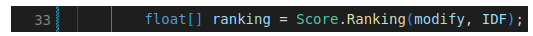
\includegraphics[height = 0.8 cm ]{Captura desde 2023-07-19 11-41-47.png}

\

En la línea 35 se inicializa el diccionario para que no presente un error al ejecutar el proyecto.

\

\centering
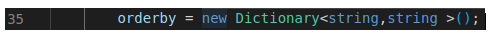
\includegraphics[height = 0.8 cm ]{Captura desde 2023-07-19 11-48-50.png}

\

De la línea 36 a la 40 se crea un for en el cual se va iterando sobre el array ranking con el objetivo de llenar los diccionarios "order" y "orderby".
En la llave del diccionario "order" guardamos el nombre de cada documento correspondiente al valor que contiene en el ranking y en el diccionario "orderby" guardamos el diccionario "order" 
y en la llave se guarda el cuerpo del documento correspondiente.

\

\centering
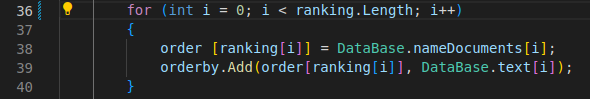
\includegraphics[height = 2 cm ]{Captura desde 2023-07-20 00-12-13.png}

\

Las líneas 42 y 43 tienen como objetivo ordenar el ranking de los documentos, el primer método lo que hace ordenar los escores de menos a mayor y el segundo invertir el orden, para que sea de 
mayor a menor, esto es para que cuando se haga la búsqueda muestre los documentos que mayor coincidencia tienen con la query se muestren de primeros .

\

\centering
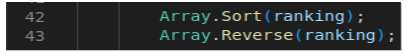
\includegraphics[height = 1 cm ]{Captura desde 2023-07-19 11-52-28.png}

\

El bloque de código siguiente tiene como objetivo que: Si el mayor “score”(importancia de un documento con la query) es 0 entonces devolverá un mensaje.

\

\centering
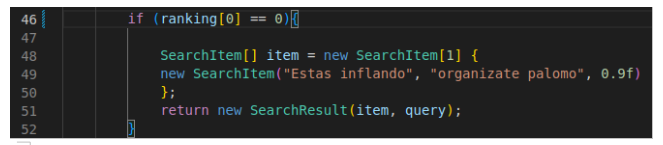
\includegraphics[height = 2.5 cm ]{Captura desde 2023-07-19 11-55-34.png}

\

En caso que el “score” sea distinto de 0 entonces se ejecuta el for el cual en la variable “snippet” se guardará un fragmento de texto del documento que el usuario solicitó. Para ello se llama 
la Clase “Snippet” específicamente al método “ShowWords” y se le pasa el cuerpo de los documentos que es el diccionario “orderby”. Posteriormente a la lista “item” le agregamos el nombre de los 
textos, el snippet y su score. 

\

\centering
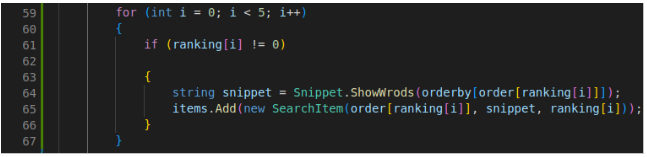
\includegraphics[height = 2.9 cm ]{Captura desde 2023-07-19 12-13-44.png}

\

Finalmente en la linea 69 se devuelven los resultados 

\

\centering
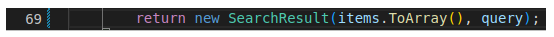
\includegraphics[height = 0.8 cm ]{Captura desde 2023-07-19 12-17-54.png}

}
\end{document}